\documentclass{article}\usepackage[]{graphicx}\usepackage[]{color}
%% maxwidth is the original width if it is less than linewidth
%% otherwise use linewidth (to make sure the graphics do not exceed the margin)
\makeatletter
\def\maxwidth{ %
  \ifdim\Gin@nat@width>\linewidth
    \linewidth
  \else
    \Gin@nat@width
  \fi
}
\makeatother

\definecolor{fgcolor}{rgb}{0.345, 0.345, 0.345}
\newcommand{\hlnum}[1]{\textcolor[rgb]{0.686,0.059,0.569}{#1}}%
\newcommand{\hlstr}[1]{\textcolor[rgb]{0.192,0.494,0.8}{#1}}%
\newcommand{\hlcom}[1]{\textcolor[rgb]{0.678,0.584,0.686}{\textit{#1}}}%
\newcommand{\hlopt}[1]{\textcolor[rgb]{0,0,0}{#1}}%
\newcommand{\hlstd}[1]{\textcolor[rgb]{0.345,0.345,0.345}{#1}}%
\newcommand{\hlkwa}[1]{\textcolor[rgb]{0.161,0.373,0.58}{\textbf{#1}}}%
\newcommand{\hlkwb}[1]{\textcolor[rgb]{0.69,0.353,0.396}{#1}}%
\newcommand{\hlkwc}[1]{\textcolor[rgb]{0.333,0.667,0.333}{#1}}%
\newcommand{\hlkwd}[1]{\textcolor[rgb]{0.737,0.353,0.396}{\textbf{#1}}}%
\let\hlipl\hlkwb

\usepackage{framed}
\makeatletter
\newenvironment{kframe}{%
 \def\at@end@of@kframe{}%
 \ifinner\ifhmode%
  \def\at@end@of@kframe{\end{minipage}}%
  \begin{minipage}{\columnwidth}%
 \fi\fi%
 \def\FrameCommand##1{\hskip\@totalleftmargin \hskip-\fboxsep
 \colorbox{shadecolor}{##1}\hskip-\fboxsep
     % There is no \\@totalrightmargin, so:
     \hskip-\linewidth \hskip-\@totalleftmargin \hskip\columnwidth}%
 \MakeFramed {\advance\hsize-\width
   \@totalleftmargin\z@ \linewidth\hsize
   \@setminipage}}%
 {\par\unskip\endMakeFramed%
 \at@end@of@kframe}
\makeatother

\definecolor{shadecolor}{rgb}{.97, .97, .97}
\definecolor{messagecolor}{rgb}{0, 0, 0}
\definecolor{warningcolor}{rgb}{1, 0, 1}
\definecolor{errorcolor}{rgb}{1, 0, 0}
\newenvironment{knitrout}{}{} % an empty environment to be redefined in TeX

\usepackage{alltt}

\usepackage{graphicx}
\usepackage{float}
\usepackage{amsmath}
\usepackage{mathtools}
\usepackage{blindtext}
\usepackage[inline]{enumitem}
\usepackage{xcolor}
\usepackage{bm}
\usepackage {fancyvrb}
\usepackage {listings}
\usepackage[makeroom]{cancel}
\IfFileExists{upquote.sty}{\usepackage{upquote}}{}
\begin{document}


\title{Sampling the Pair Potential Space}
\maketitle

In this case we have two MeOH molecules separated by 5\AA\ in the $y$ direction.

\begin{figure}[H]
  \center
  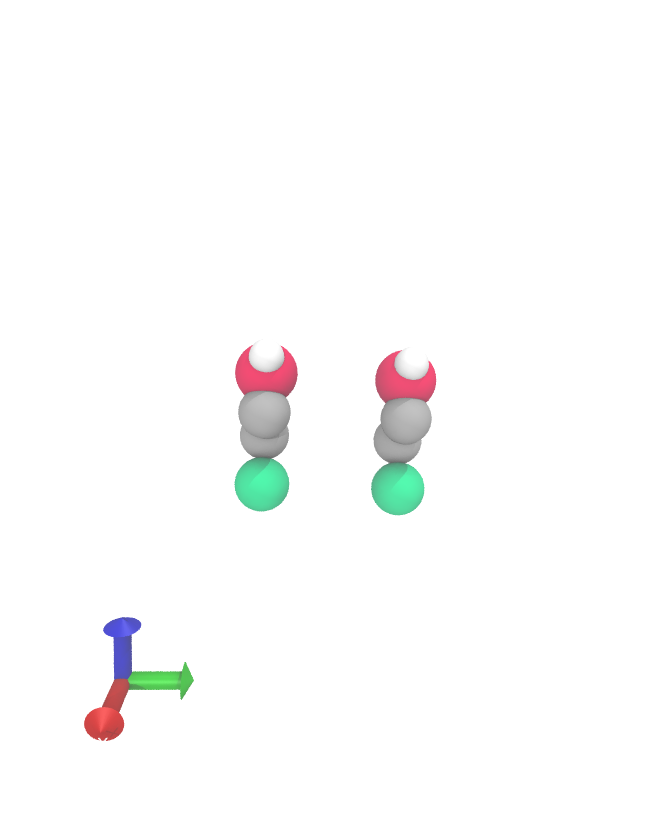
\includegraphics[trim=0 0 0 300,clip,width=0.5\textwidth]{two_meoh}
\end{figure}

Our MeOH molecules have the following coordinates:

\begin{align*}
  &S\ (0.138,0.0,-1.654)   &S'\ (0.138,5.0,-1.654)\\
  &C1\ (0.474,0.0,1.059)   &C1'\ (0.474,5.0,1.059)\\
  &C2\ (-0.621,0.0,-0.007) &C2'\ (-0.621,5.0,-0.007)\\
  &O\ (-0.125,0.0,2.357)   &O'\ (-0.125,5.0,2.357)\\
  &H\ (0.598,0.0,2.999)    &H'\ (0.598,5.0,2.999)\\
\end{align*}

\begin{knitrout}
\definecolor{shadecolor}{rgb}{0.969, 0.969, 0.969}\color{fgcolor}\begin{kframe}
\begin{alltt}
  \hlstd{S}\hlkwb{=}\hlkwd{c}\hlstd{(}\hlnum{2}\hlstd{,}\hlnum{0.0}\hlstd{,}\hlnum{0.138}\hlstd{,}\hlnum{0.0}\hlstd{,}\hlopt{-}\hlnum{1.654}\hlstd{)}
  \hlstd{C1}\hlkwb{=}\hlkwd{c}\hlstd{(}\hlnum{1}\hlstd{,}\hlnum{0.0}\hlstd{,}\hlnum{0.474}\hlstd{,}\hlnum{0.0}\hlstd{,}\hlnum{1.059}\hlstd{)}
  \hlstd{C2}\hlkwb{=}\hlkwd{c}\hlstd{(}\hlnum{1}\hlstd{,}\hlnum{0.265}\hlstd{,}\hlopt{-}\hlnum{0.621}\hlstd{,}\hlnum{0.0}\hlstd{,}\hlopt{-}\hlnum{0.007}\hlstd{)}
  \hlstd{O}\hlkwb{=}\hlkwd{c}\hlstd{(}\hlnum{3}\hlstd{,}\hlopt{-}\hlnum{0.700}\hlstd{,}\hlopt{-}\hlnum{0.125}\hlstd{,}\hlnum{0.0}\hlstd{,}\hlnum{2.357}\hlstd{)}
  \hlstd{H}\hlkwb{=}\hlkwd{c}\hlstd{(}\hlnum{4}\hlstd{,}\hlnum{0.435}\hlstd{,}\hlnum{0.598}\hlstd{,}\hlnum{0.0}\hlstd{,}\hlnum{2.999}\hlstd{)}
  \hlstd{S_2}\hlkwb{=}\hlkwd{c}\hlstd{(}\hlnum{2}\hlstd{,}\hlnum{0.0}\hlstd{,}\hlnum{0.138}\hlstd{,}\hlnum{5.0}\hlstd{,}\hlopt{-}\hlnum{1.654}\hlstd{)}
  \hlstd{C1_2}\hlkwb{=}\hlkwd{c}\hlstd{(}\hlnum{1}\hlstd{,}\hlnum{0.0}\hlstd{,}\hlnum{0.474}\hlstd{,}\hlnum{5.0}\hlstd{,}\hlnum{1.059}\hlstd{)}
  \hlstd{C2_2}\hlkwb{=}\hlkwd{c}\hlstd{(}\hlnum{1}\hlstd{,}\hlnum{0.265}\hlstd{,}\hlopt{-}\hlnum{0.621}\hlstd{,}\hlnum{5.0}\hlstd{,}\hlopt{-}\hlnum{0.007}\hlstd{)}
  \hlstd{O_2}\hlkwb{=}\hlkwd{c}\hlstd{(}\hlnum{3}\hlstd{,}\hlopt{-}\hlnum{0.700}\hlstd{,}\hlopt{-}\hlnum{0.125}\hlstd{,}\hlnum{5.0}\hlstd{,}\hlnum{2.357}\hlstd{)}
  \hlstd{H_2}\hlkwb{=}\hlkwd{c}\hlstd{(}\hlnum{4}\hlstd{,}\hlnum{0.435}\hlstd{,}\hlnum{0.598}\hlstd{,}\hlnum{5.0}\hlstd{,}\hlnum{2.999}\hlstd{)}
\end{alltt}
\end{kframe}
\end{knitrout}

Rotating the $SCCO$ dihedral we get:

\begin{knitrout}
\definecolor{shadecolor}{rgb}{0.969, 0.969, 0.969}\color{fgcolor}\begin{kframe}
\begin{alltt}
  \hlkwd{library}\hlstd{(onion)}
  \hlstd{axis} \hlkwb{=} \hlstd{C2[}\hlnum{3}\hlopt{:}\hlnum{5}\hlstd{]}\hlopt{-}\hlstd{C1[}\hlnum{3}\hlopt{:}\hlnum{5}\hlstd{]}
  \hlstd{normaxis} \hlkwb{=} \hlstd{axis}\hlopt{/}\hlkwd{sqrt}\hlstd{(}\hlkwd{sum}\hlstd{(axis}\hlopt{^}\hlnum{2}\hlstd{))}
  \hlstd{numpoints} \hlkwb{=} \hlnum{500}
  \hlstd{theta} \hlkwb{=} \hlkwd{seq}\hlstd{(}\hlnum{0}\hlstd{,}\hlnum{2}\hlopt{*}\hlstd{pi,}\hlkwc{length.out} \hlstd{= numpoints)}
  \hlcom{#q = sapply(theta,function(x) cos(x/2)+sin(x/2)*normaxis[1]*Hi+sin(x/2)*normaxis[2]*Hj+sin(x/2)*normaxis[3]*Hk)}
  \hlstd{q} \hlkwb{=} \hlkwd{cos}\hlstd{(theta}\hlopt{/}\hlnum{2}\hlstd{)}\hlopt{+}\hlkwd{sin}\hlstd{(theta}\hlopt{/}\hlnum{2}\hlstd{)}\hlopt{*}\hlstd{normaxis[}\hlnum{1}\hlstd{]}\hlopt{*}\hlstd{Hi}\hlopt{+}\hlkwd{sin}\hlstd{(theta}\hlopt{/}\hlnum{2}\hlstd{)}\hlopt{*}\hlstd{normaxis[}\hlnum{2}\hlstd{]}\hlopt{*}\hlstd{Hj}\hlopt{+}\hlkwd{sin}\hlstd{(theta}\hlopt{/}\hlnum{2}\hlstd{)}\hlopt{*}\hlstd{normaxis[}\hlnum{3}\hlstd{]}\hlopt{*}\hlstd{Hk}
  \hlcom{#print(q)}
\end{alltt}
\end{kframe}
\end{knitrout}

\begin{knitrout}
\definecolor{shadecolor}{rgb}{0.969, 0.969, 0.969}\color{fgcolor}\begin{kframe}
\begin{alltt}
\hlstd{v1} \hlkwb{=} \hlstd{O[}\hlnum{3}\hlopt{:}\hlnum{5}\hlstd{]} \hlopt{-} \hlstd{C2[}\hlnum{3}\hlopt{:}\hlnum{5}\hlstd{]}
\hlstd{v2} \hlkwb{=} \hlstd{H[}\hlnum{3}\hlopt{:}\hlnum{5}\hlstd{]} \hlopt{-} \hlstd{C2[}\hlnum{3}\hlopt{:}\hlnum{5}\hlstd{]}
\hlstd{v1_q} \hlkwb{=} \hlnum{0} \hlopt{+} \hlstd{v1[}\hlnum{1}\hlstd{]} \hlopt{*} \hlstd{Hi} \hlopt{+} \hlstd{v1[}\hlnum{2}\hlstd{]} \hlopt{*} \hlstd{Hj} \hlopt{+} \hlstd{v1[}\hlnum{3}\hlstd{]} \hlopt{*} \hlstd{Hk}
\hlstd{v2_q} \hlkwb{=} \hlnum{0} \hlopt{+} \hlstd{v2[}\hlnum{1}\hlstd{]} \hlopt{*} \hlstd{Hi} \hlopt{+} \hlstd{v2[}\hlnum{2}\hlstd{]} \hlopt{*} \hlstd{Hj} \hlopt{+} \hlstd{v2[}\hlnum{3}\hlstd{]} \hlopt{*} \hlstd{Hk}
\hlstd{v1_rot_q} \hlkwb{=} \hlstd{q} \hlopt{*} \hlstd{v1_q} \hlopt{*} \hlkwd{Conj}\hlstd{(q)}
\hlstd{v2_rot_q} \hlkwb{=} \hlstd{q} \hlopt{*} \hlstd{v2_q} \hlopt{*} \hlkwd{Conj}\hlstd{(q)}
\hlstd{v1_rot} \hlkwb{=} \hlkwd{data.frame}\hlstd{(}\hlkwc{x} \hlstd{=} \hlkwd{i}\hlstd{(v1_rot_q),} \hlkwc{y} \hlstd{=} \hlkwd{j}\hlstd{(v1_rot_q),} \hlkwc{z} \hlstd{=} \hlkwd{k}\hlstd{(v1_rot_q))}
\hlstd{v2_rot} \hlkwb{=} \hlkwd{data.frame}\hlstd{(}\hlkwc{x} \hlstd{=} \hlkwd{i}\hlstd{(v2_rot_q),} \hlkwc{y} \hlstd{=} \hlkwd{j}\hlstd{(v2_rot_q),} \hlkwc{z} \hlstd{=} \hlkwd{k}\hlstd{(v2_rot_q))}
\hlcom{# print(v1_rot)}
\hlstd{Onew} \hlkwb{=} \hlstd{v1_rot} \hlopt{+} \hlkwd{matrix}\hlstd{(}\hlkwd{rep}\hlstd{(C2[}\hlnum{3}\hlopt{:}\hlnum{5}\hlstd{],} \hlkwc{times} \hlstd{= numpoints),} \hlkwc{ncol} \hlstd{=} \hlnum{3}\hlstd{,} \hlkwc{byrow} \hlstd{=} \hlnum{TRUE}\hlstd{)}
\hlstd{Hnew} \hlkwb{=} \hlstd{v2_rot} \hlopt{+} \hlkwd{matrix}\hlstd{(}\hlkwd{rep}\hlstd{(C2[}\hlnum{3}\hlopt{:}\hlnum{5}\hlstd{],} \hlkwc{times} \hlstd{= numpoints),} \hlkwc{ncol} \hlstd{=} \hlnum{3}\hlstd{,} \hlkwc{byrow} \hlstd{=} \hlnum{TRUE}\hlstd{)}
\hlcom{# print(Onew) print(Hnew)}
\end{alltt}
\end{kframe}
\end{knitrout}

\begin{knitrout}
\definecolor{shadecolor}{rgb}{0.969, 0.969, 0.969}\color{fgcolor}\begin{kframe}
\begin{alltt}
  \hlstd{epsilons}\hlkwb{=}\hlkwd{c}\hlstd{(}\hlnum{0.118}\hlstd{,}\hlnum{0.39743}\hlstd{,}\hlnum{0.20}\hlstd{,}\hlnum{0.000}\hlstd{)}
  \hlstd{sigmas}\hlkwb{=}\hlkwd{c}\hlstd{(}\hlnum{3.905}\hlstd{,}\hlnum{4.25}\hlstd{,}\hlnum{2.85}\hlstd{,}\hlnum{1.78}\hlstd{)}
  \hlstd{distance}\hlkwb{=}\hlkwa{function}\hlstd{(}\hlkwc{atom1}\hlstd{,}\hlkwc{atom2}\hlstd{)\{}
    \hlkwd{return}\hlstd{(}\hlkwd{norm}\hlstd{(atom1[}\hlnum{3}\hlopt{:}\hlnum{5}\hlstd{]}\hlopt{-}\hlstd{atom2[}\hlnum{3}\hlopt{:}\hlnum{5}\hlstd{],}\hlkwc{type}\hlstd{=}\hlstr{"2"}\hlstd{))}
  \hlstd{\}}
  \hlstd{energy}\hlkwb{=}\hlkwa{function}\hlstd{(}\hlkwc{atom1}\hlstd{,}\hlkwc{atom2}\hlstd{)\{}
    \hlstd{r}\hlkwb{=}\hlkwd{distance}\hlstd{(atom1,atom2)}
    \hlstd{sigma} \hlkwb{=} \hlstd{(sigmas[atom1[}\hlnum{1}\hlstd{]]}\hlopt{+}\hlstd{sigmas[atom2[}\hlnum{1}\hlstd{]])}\hlopt{/}\hlnum{2}
    \hlstd{epsilon} \hlkwb{=} \hlkwd{sqrt}\hlstd{(epsilons[atom1[}\hlnum{1}\hlstd{]]}\hlopt{*}\hlstd{epsilons[atom2[}\hlnum{1}\hlstd{]])}
    \hlkwd{return}\hlstd{(}\hlnum{4}\hlopt{*}\hlstd{epsilon}\hlopt{*}\hlstd{((sigma}\hlopt{/}\hlstd{r)}\hlopt{^}\hlnum{12}\hlopt{-}\hlstd{(sigma}\hlopt{/}\hlstd{r)}\hlopt{^}\hlnum{6}\hlstd{))}
  \hlstd{\}}
  \hlstd{coul_energy}\hlkwb{=}\hlkwa{function}\hlstd{(}\hlkwc{atom1}\hlstd{,}\hlkwc{atom2}\hlstd{)\{}
    \hlstd{r}\hlkwb{=}\hlkwd{distance}\hlstd{(atom1,atom2)}
    \hlstd{k}\hlkwb{=}\hlnum{0.2}
    \hlkwd{return}\hlstd{(}\hlnum{332.0636}\hlopt{*}\hlstd{((atom1[}\hlnum{2}\hlstd{]}\hlopt{*}\hlstd{atom2[}\hlnum{2}\hlstd{])}\hlopt{/}\hlstd{r)}\hlopt{*}\hlkwd{exp}\hlstd{(}\hlopt{-}\hlstd{k}\hlopt{*}\hlstd{r))}
  \hlstd{\}}
  \hlcom{#atoms = list(S,C1,C2,O,H,S_2,C1_2,C2_2,O_2,H_2)}
  \hlstd{atoms} \hlkwb{=} \hlkwd{list}\hlstd{(S,C1,C2,O,S_2,C1_2,C2_2,O_2,H_2)}
  \hlstd{atom_combos} \hlkwb{=} \hlkwd{combn}\hlstd{(atoms,}\hlnum{2}\hlstd{)}
  \hlstd{distances}\hlkwb{=}\hlkwd{mapply}\hlstd{(distance,atom_combos[}\hlnum{1}\hlstd{,],atom_combos[}\hlnum{2}\hlstd{,])}
  \hlstd{indices}\hlkwb{=}\hlstd{distances}\hlopt{>=}\hlnum{5}
  \hlstd{total_energy}\hlkwb{=}\hlkwa{function}\hlstd{(}\hlkwc{atoms}\hlstd{)\{}
    \hlstd{atom_combos} \hlkwb{=} \hlkwd{combn}\hlstd{(atoms,}\hlnum{2}\hlstd{)}
    \hlstd{distances}\hlkwb{=}\hlkwd{mapply}\hlstd{(distance,atom_combos[}\hlnum{1}\hlstd{,],atom_combos[}\hlnum{2}\hlstd{,])}
    \hlstd{vdw_energies} \hlkwb{=} \hlkwd{mapply}\hlstd{(energy,atom_combos[,indices][}\hlnum{1}\hlstd{,],atom_combos[,indices][}\hlnum{2}\hlstd{,])}
    \hlstd{coul_energies} \hlkwb{=} \hlkwd{mapply}\hlstd{(coul_energy,atom_combos[,indices][}\hlnum{1}\hlstd{,],atom_combos[,indices][}\hlnum{2}\hlstd{,])}
    \hlkwd{return}\hlstd{(}\hlkwd{sum}\hlstd{(vdw_energies)}\hlopt{+}\hlkwd{sum}\hlstd{(coul_energies))}
  \hlstd{\}}
  \hlstd{apply_energy} \hlkwb{=} \hlkwa{function}\hlstd{(}\hlkwc{Onew}\hlstd{,}\hlkwc{Hnew}\hlstd{)\{}
    \hlcom{#print(Onew[1:3])}
    \hlcom{#print(atoms[[4]][3:5])}
    \hlstd{atoms[[}\hlnum{4}\hlstd{]][}\hlnum{3}\hlopt{:}\hlnum{5}\hlstd{]} \hlkwb{=} \hlkwd{c}\hlstd{(Onew}\hlopt{$}\hlstd{x,Onew}\hlopt{$}\hlstd{y,Onew}\hlopt{$}\hlstd{z)}
    \hlcom{#print(atoms[[4]][3:5])}
    \hlcom{#atoms[[5]][3:5] = c(Hnew$x,Hnew$y,Hnew$z)}
    \hlstd{atom_combos} \hlkwb{=} \hlkwd{combn}\hlstd{(atoms,}\hlnum{2}\hlstd{)}
    \hlstd{distances}\hlkwb{=}\hlkwd{mapply}\hlstd{(distance,atom_combos[}\hlnum{1}\hlstd{,],atom_combos[}\hlnum{2}\hlstd{,])}
    \hlstd{vdw_energies} \hlkwb{=} \hlkwd{mapply}\hlstd{(energy,atom_combos[,indices][}\hlnum{1}\hlstd{,],atom_combos[,indices][}\hlnum{2}\hlstd{,])}
    \hlstd{coul_energies} \hlkwb{=} \hlkwd{mapply}\hlstd{(coul_energy,atom_combos[,indices][}\hlnum{1}\hlstd{,],atom_combos[,indices][}\hlnum{2}\hlstd{,])}
    \hlkwd{return}\hlstd{(}\hlkwd{sum}\hlstd{(vdw_energies)}\hlopt{+}\hlkwd{sum}\hlstd{(coul_energies))}
  \hlstd{\}}
  \hlcom{#print(total_energy(atoms))}
  \hlstd{energies} \hlkwb{=} \hlkwd{sapply}\hlstd{(}\hlkwd{seq}\hlstd{(}\hlnum{1}\hlstd{,numpoints),}\hlkwa{function}\hlstd{(}\hlkwc{i}\hlstd{)} \hlkwd{apply_energy}\hlstd{(Onew[i,],Hnew[i,]))}
  \hlkwd{plot}\hlstd{(theta,energies}\hlopt{-}\hlstd{energies[}\hlnum{1}\hlstd{])}
\end{alltt}
\end{kframe}
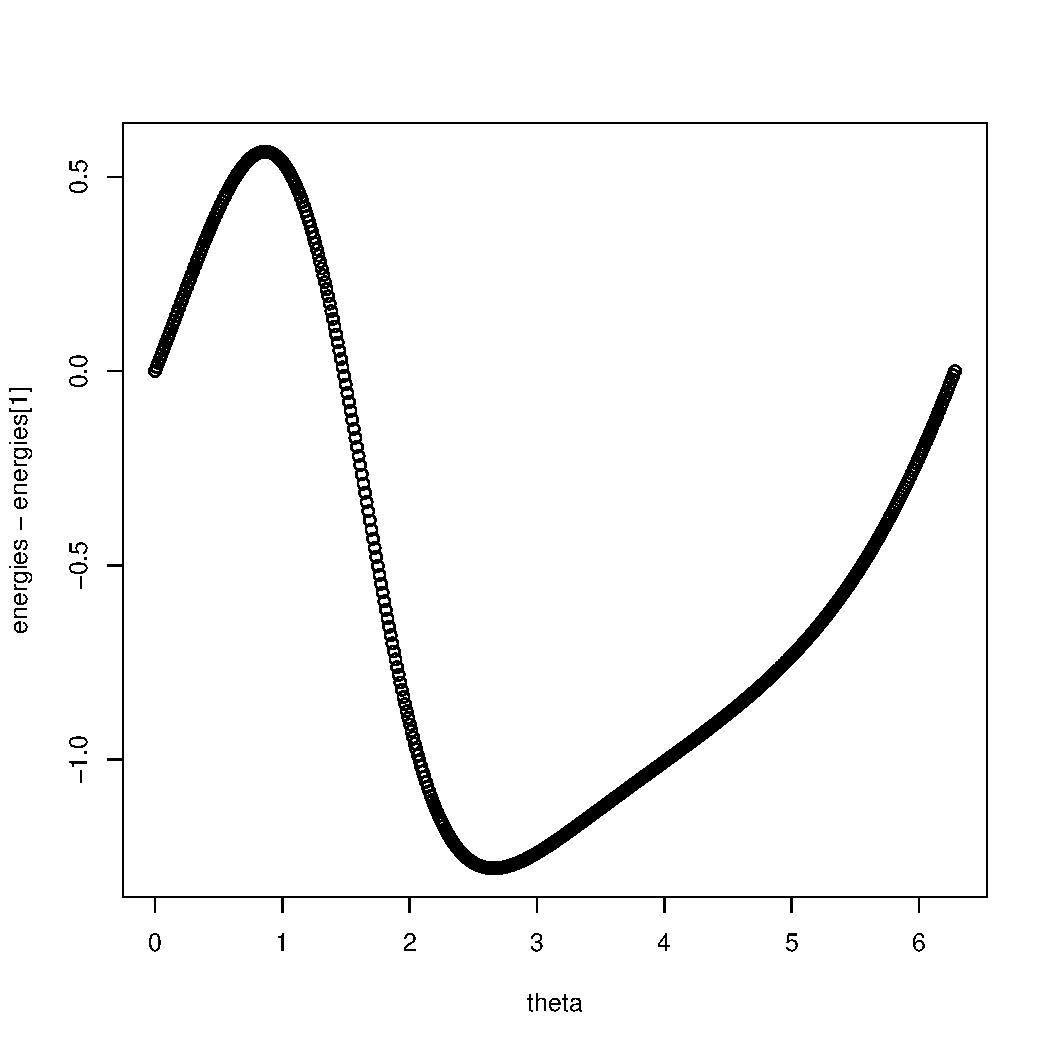
\includegraphics[width=\maxwidth]{figure/combinations-1} 

\end{knitrout}

Calculating the probabilities we get:

\begin{knitrout}
\definecolor{shadecolor}{rgb}{0.969, 0.969, 0.969}\color{fgcolor}\begin{kframe}
\begin{alltt}
  \hlstd{Temp} \hlkwb{=} \hlnum{298.15}
  \hlstd{kb} \hlkwb{=} \hlnum{0.0019872041}
  \hlstd{beta} \hlkwb{=} \hlnum{1.}\hlopt{/}\hlstd{(kb}\hlopt{*}\hlstd{Temp)}
  \hlstd{dtheta} \hlkwb{=} \hlstd{theta[}\hlnum{2}\hlstd{]}\hlopt{-}\hlstd{theta[}\hlnum{1}\hlstd{]}
  \hlstd{probs} \hlkwb{=} \hlkwd{exp}\hlstd{(}\hlopt{-}\hlstd{beta}\hlopt{*}\hlstd{(energies}\hlopt{-}\hlstd{energies[}\hlnum{1}\hlstd{]))}
  \hlstd{norm_probs} \hlkwb{=} \hlstd{probs}\hlopt{/}\hlstd{(}\hlkwd{sum}\hlstd{(probs)}\hlopt{*}\hlstd{dtheta)}
  \hlkwd{plot}\hlstd{(theta,norm_probs)}
\end{alltt}
\end{kframe}
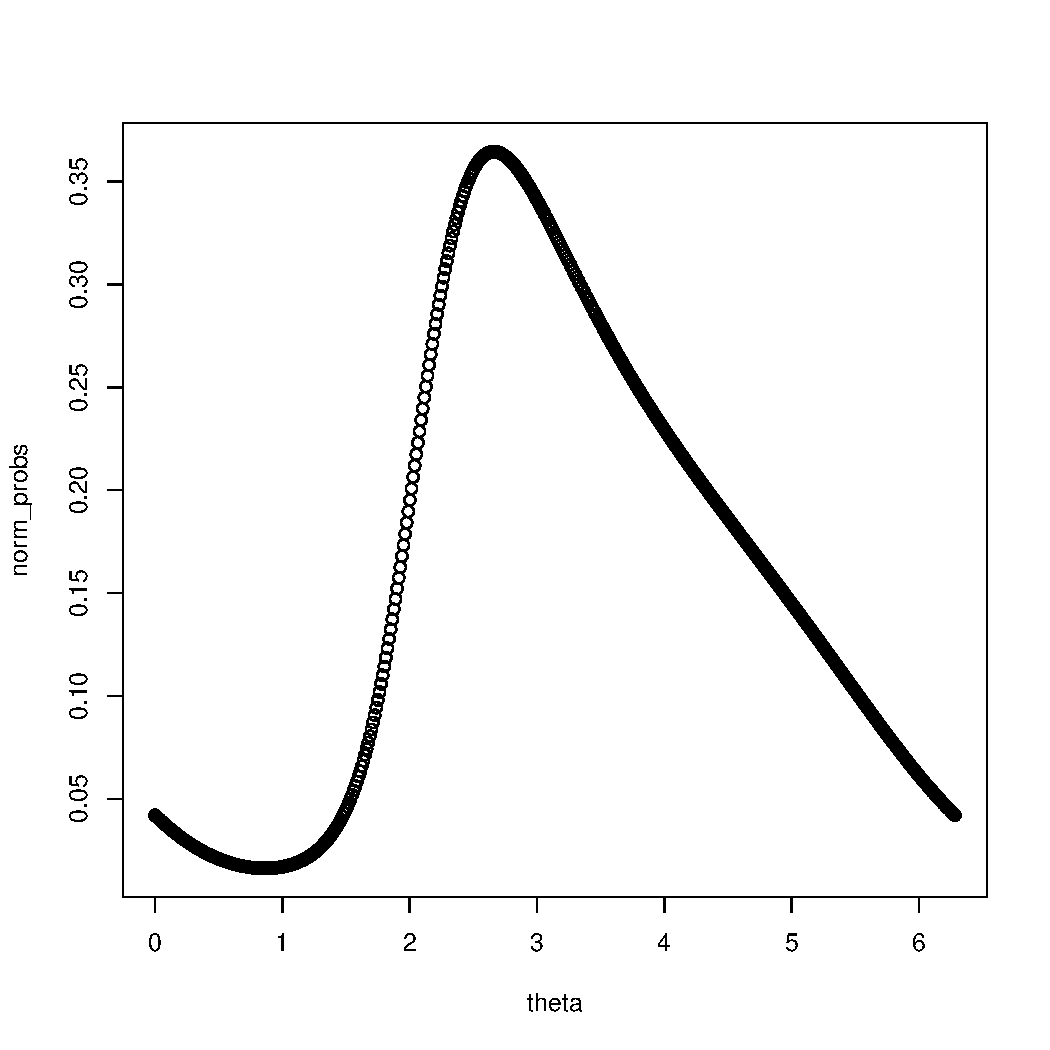
\includegraphics[width=\maxwidth]{figure/probabilities-1} 
\begin{kframe}\begin{alltt}
  \hlkwd{write.csv}\hlstd{(norm_probs,}\hlkwc{file} \hlstd{=} \hlstr{"pair_pe_pdf.csv"}\hlstd{,}\hlkwc{row.names} \hlstd{=} \hlnum{FALSE}\hlstd{,}\hlkwc{col.names} \hlstd{=} \hlnum{FALSE}\hlstd{)}
\end{alltt}


{\ttfamily\noindent\color{warningcolor}{\#\# Warning in write.csv(norm\_probs, file = "{}pair\_pe\_pdf.csv"{}, row.names = FALSE, : attempt to set 'col.names' ignored}}\end{kframe}
\end{knitrout}


\end{document}















